%!TEX root = proj_report_outline.tex
\chapter{Threshold Security Scheme}\label{C:threshholdSecurity}

\section{Design}
As discussed in Section \ref{S:databaseSecurity} Shamir's Secret Sharing Scheme is a threshold security scheme based on Lagrange interpolation. Recall, the scheme works by splitting the secret into \textit{n} shares, \textit{k} of which are required to then retrieve the original secret. In this section the design for the service enabling PitchHub to leverage the secret sharing scheme is discussed.

\subsection{Shamir's Secret Sharing Scheme Service}\label{SS:design_shamir_secret_sharing_service}
First, in designing the service an open-source implementation of Shamir's Secret Sharing was selected. This was a key design decision. While the principles of Shamir's Secret Sharing are simple, personally implementing a cryptography library should be treated with care. To implement and establish trust in such a component would require rigorous testing to be proven as secure. Leveraging the collective strength of the open-source community ensures that the implementations have had many eyes go through them (with different backgrounds/expertises). The primary activity for PitchHub in regards to Secret Sharing was to design and implement a service that integrates the security scheme.
\par
As discussed by prominent cryptographer and author \citeauthor{schneier1999cryptography} ``Building cryptography into products is hard... Flaws can appear anywhere. They can be in the trust model, the system design, the algorithms and protocols, the implementations, the source code, the human-computer interface, the procedures, the underlying computer system. Anywhere.'' \cite{schneier1999cryptography}. PitchHub  approached the integration of the security scheme library with emphasis on limiting the amount of coupling. By reducing coupling between the library and wider system we reduce the risk of system knowledge producing vulnerabilities within PitchHub and undermining the security scheme's integrity.
\par
In designing this service the MVC architecture pattern was analysed in regards to which component is most suitable to handle this responsibility. The model could use a Ruby mixin to override both it's \textit{save} and \textit{find} methods such that the secret was split into \textit{n} shares on \textit{save} for the \textit{n} databases. \textit{Find} would work similarly, merely combining the queried shares from the \textit{k..n} databases and presenting the clear text secret. The view component is not supposed to deal with business logic and hence not an appropriate candidate for this responsibility. The controller in it's capacity of delegating tasks to models could also bear this responsibility. In the controller on \textit{saves} it could split the secret among \textit{n} models and save each model to a distinct database. With \textit{finds} the controller would need to connect to each database and retrieve the requested secrets to combine. The pros and cons of each design is apparent. Going strictly the model route would mean \textit{monkey patching} \cite{Monke1:online} the behaviour of the ODM which could make it hard for other components that do not wish to use the Secret Sharing implementation also this would require that models have knowledge outside of itself. Going strictly controller means that there is a fair amount of business logic within the controllers. However, both approaches consolidate the integration of the Secret Sharing library within it's own component. Ultimately, the final approach was a mixture of the above, controllers were modified such that they use explicit Secret Sharing \textit{find} and \textit{save} methods which encapsulate the knowledge of the \textit{n} secret keeper databases, within these explicit Secret Sharing database methods the logic of the Secret Sharing library is isolated.
\par
Despite both Models and Controllers being aware of the Secret Sharing functionality, they are only aware of as much to the capacity of their roles. The model handles the business logic, while the controller handles the delegation.

\subsection{Overcoming Limitations of Threshold Security Schemes}
Given share combinations up to \textit{k}, Secret Sharing Schemes ensure that the secret's safety is maintained. However, if an attacker gains \textit{k} secret shares, the secret is easily reconstructed. This is simultaneously the advantage and weakness of Threshold Security Schemes. To explore further in the context of PitchHub: up to \textit{k} compromised databases do not compromise the security of the secrets being held, but if an attacker is able to break into one database it is reasonable to infer that they are capable of breaking into all of them. Furthermore this scheme relies on the availability of \textit{k} secret keepers, should \textit{k} be unattainable the secrets are rendered irretrievable to both authorised and unauthorised users alike.
\par
The first issue can be alleviated by introducing diversity to the secret keepers. Instead of all secret keepers being MongoDB instances including alternative data stores in the secret keeper configuration means that the vulnerabilities of the data stores themselves do not manifest as a vulnerability for the system as a whole. However, to do this effectively we require a configuration where there is not \textit{k} secret keepers of the same data store. If there were, the whole exercise of including alternative data stores would be rendered moot as an attacker with the ability to breach the particular data store would be able to fulfil the threshold \textit{k}. This issue of diversity and security is explored by \citeauthor{littlewood2004redundancy} who conclude that depending on the context diversity can be one of the most effective means of neutralising `systemic' attacks by merely avoiding the danger.
\par
There is a fundamental tension in the relationship between availability and security in threshold schemes. Representations of the classic Threshold Security Schemes where each secret keeper contains one and only share of the secret favour security over availability. This is great when secret keepers do not have any membership changes or only member changes that still preserve \textit{k} secret keepers. In this example should \textit{k} or more secret keepers go down the entire service becomes unavailable, and in cases where \textit{k} cannot ever be re-established then the secret data is irretrievable. There are a number of approaches that can be used to increase availability but each suffer from an increase in complexity and a decrease in security. For example, concepts used in distributed databases are directly applicable to secret sharing schemes. Redundancy and hinted hand-off are methods used by distributed database systems are used to ensure availability by node's sharing their data such that if they go down the data stored is still accessible through the nodes who hold the shared data. In the context of Threshold Schemes this means that some nodes may have more than one secret share for the same secret, this demonstrably reduces the significance of the threshold. For a system like PitchHub I believe classic redundancy where each member would contain a whole other keeper's secret shares is a step too far. However we could raise availability of the secret members themselves by representing secret members as high-availability clusters rather than individual databases, this architecture configuration is featured in Fig \ref{fig:architecture_high_availability}.

\begin{figure}[ht]
    \centering
    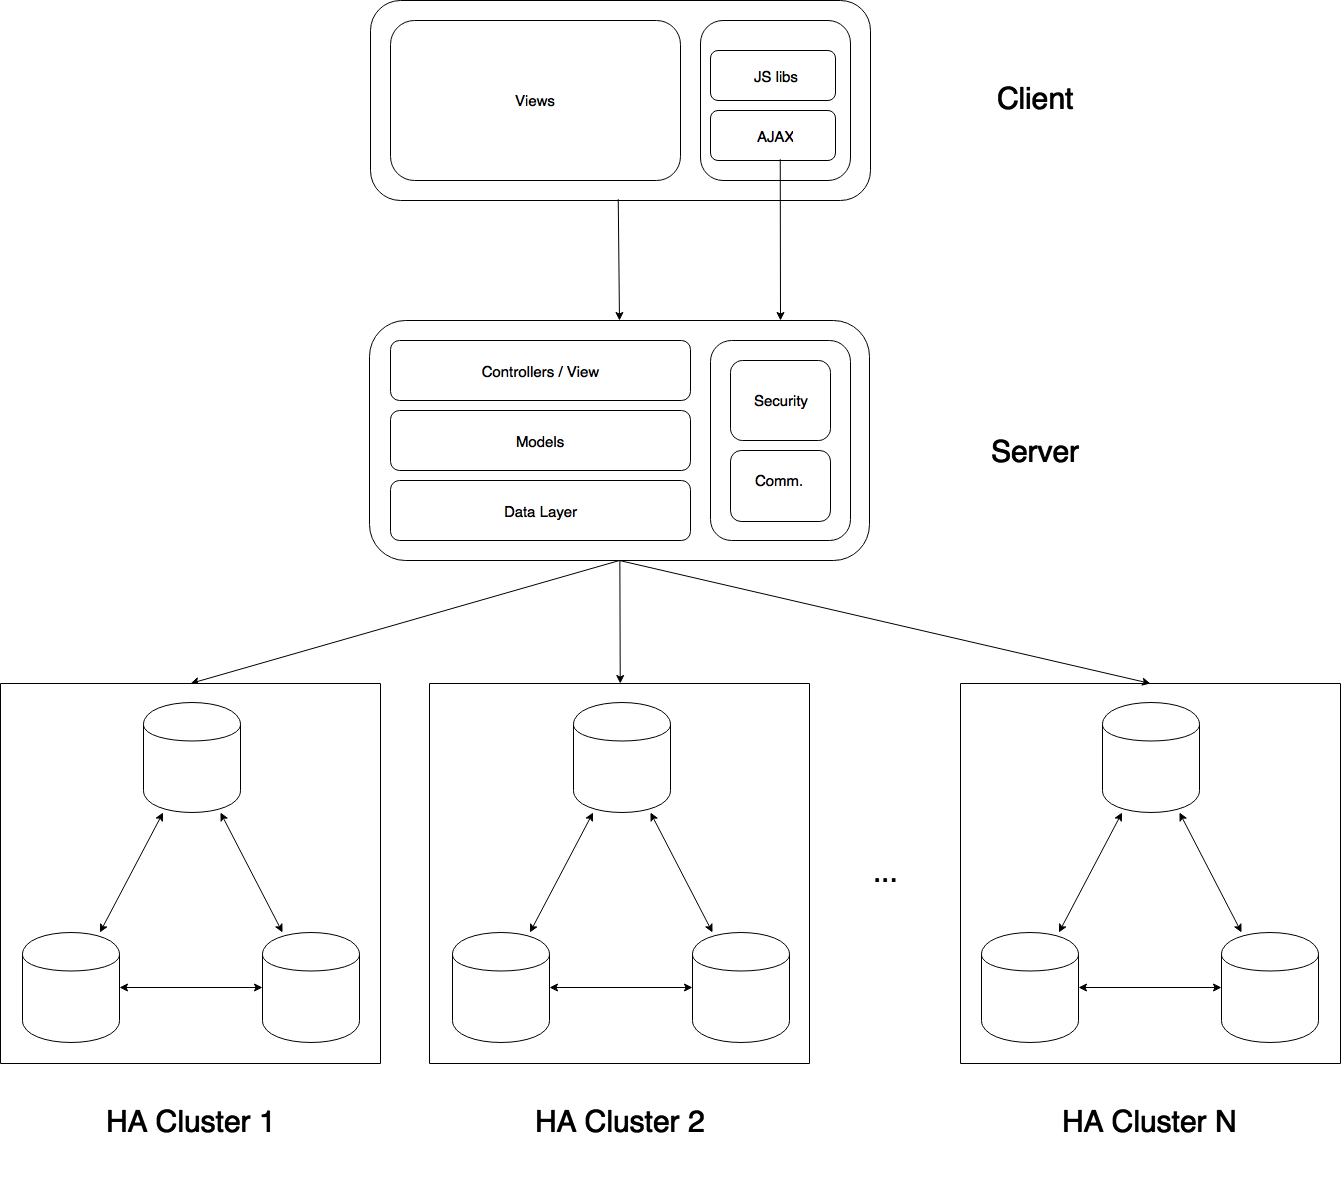
\includegraphics[width=1\textwidth]{architecture_high_availability}
    \caption{The architecture extended with high-availability clusters increases the Threshold Scheme's robustness without compromising security.}
    \label{fig:architecture_high_availability}
\end{figure}

\section{Implementation}

\subsection{Shamir's Secret Sharing Scheme Service}
The secret sharing configuration developed for the prototype used a (\textit{3},\textit{4})-threshold scheme, where at least 3 of the 4 shares representing a secret must be combined to reconstruct the secret. The technologies used for the Secret Keepers are as follows: 2x MongoDB instances, 2x PostgreSQL instances, diversity in relation to implementation is further explored in Subsection \ref{SS:diverse_secret_keepers}. The Secret Sharing Service was implemented as designed in Subsection \ref{SS:design_shamir_secret_sharing_service} to support all CRUD operations. The approach for splitting objects was done on the field level, where each object's values where split and then placed into a new object representing the share that is ultimately persisted. For example, Fig

\subsection{Diverse Secret Keepers}\label{SS:diverse_secret_keepers}



















